\subsection{\texorpdfstring{\(\mathbf{R}^n\) 的闭子群}{R 的 n 次幂的闭子群}}

我们已经知道 \(\mathbf{R}^n\) 的闭子群的两种类型：一方面是 \(\mathbf{R}^n\) 的向量子空间，它们同构于群 \(\mathbf{R}^p\) （ \(p \leqslant n\) ）（第 IV 章 § 1 第 4 小节命题 2）；另一方面是离散子群（第 III 章 § 2 第 1 小节命题 5），如我们刚才所见，它们同构于群 \(\mathbf{Z}^q\) （ \(q \leqslant n\) ）。现在我们要确定 \(\mathbf{R}^n\) 的任意闭子群的结构，办法是证明这样一个子群同构于形如

\[
\mathbf {R} ^ {p} \times \mathbf {Z} ^ {q} \quad \text { where } \quad \mathrm{o} \leqslant p + q \leqslant n.
\]

证明基于下面的命题：

命题 3. \(\mathbf{R}^n\) 的每个非离散的闭子群都包含一条过 o 的直线。

设 \((\pmb{x}_p)_{p\in \mathbb{N}}\) 是 \(\mathbf{G}\) 的点的一个无穷序列，满足 \(\pmb{x}_p\neq 0\) 且 \(\lim_{p\to \infty}\pmb{x}_p = 0\) ；由假设这样的序列存在。设 \(\mathbf{P}\) 是以 \(0\) 为中心且包含诸 \(\pmb{x}_p\) 的开立方体。设 \(k_{p}\) 表示最大的整数 \(h > 0\) ，它使 \(h\pmb{x}_p\in \mathrm{P}\) （由于 \(\mathbf{P}\) 是有界长方体且 \(\pmb{x}_p\neq 0\) ， \(k_{p}\) 的存在性由阿基米德公理得出）。点 \(k_{p}\pmb{x}_{p}\) 位于紧集 \(\overline{\mathrm{P}}\) 中，因此序列 \((k_{p}\pmb{x}_{p})_{p\in \mathbb{N}}\) 有一个聚点 \(\pmb {a}\in \overline{\mathrm{P}}\) 。若 \(||k_p\pmb {x}_p - \pmb {a}||\leqslant \varepsilon\) ，我们有

\[
\left| \left| \left(k _ {p} + \mathrm{I}\right) x _ {p} - a \right| \right| \leqslant \varepsilon + \left| \left| x _ {p} \right| \right|,
\]

且由于 \(\lim_{p\to \infty}\boldsymbol{x}_p = 0\) ，由此得出 \(\boldsymbol{a}\) 也是序列 \(((k_p + 1)x_p)\) 的一个聚点，而这个序列的点属于闭集 \(\mathfrak{C}P\) （按 \(k_{p}\) 的定义）；因此 \(\boldsymbol{a} \in \overline{\mathrm{P}} \cap \mathfrak{C}P\) （即 P 的边界，见图 5），这蕴涵 \(\boldsymbol{a} \neq 0\) 。此外，由于 G 是闭的，我们有 \(\boldsymbol{a} \in \mathrm{G}\) 。设 \(t\) 是任意实数；由于 \(|tk_p - [tk_p]| < 1\) ，关系 \(||k_p x_p - a|| \leqslant \varepsilon\) 蕴涵 \(||[tk_p]x_p - ta|| \leqslant |t| \varepsilon + ||x_p||\) ；由于 \(\lim_{p \to \infty} x_p = 0\) ， \(ta\) 是

\pandocbounded{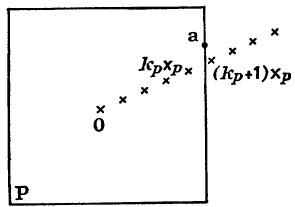
\includegraphics[keepaspectratio]{images/part001_2a0a1c84.jpg}}\\
图 5.

\pandocbounded{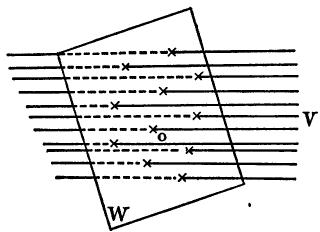
\includegraphics[keepaspectratio]{images/part001_3dc381fa.jpg}}\\
图 6.

序列 \(([tk_p]x_p)\) 的一个聚点；但这个序列的点都属于 G，因而 \(ta \in G\) ，因为 G 是闭的。证毕。

定理 2. 设 G 是 \(\mathbf{R}^n\) 的一个闭子群，其秩为 \(r\) （ \(0 \leqslant r \leqslant n\) ）。则存在含于 G 中的最大向量子空间 V；对每个与 V 互补的向量子空间 W，W ∩ G 是离散的，且 G 是 V 与 W ∩ G 的直和。

我们首先来确立 V 的存在性，办法是证明 G 中所有过 o 的直线的并集是一个向量子空间：事实上，由这些直线的并集生成的向量子空间与由它们生成的子群相同。群 G 是 V 与 W ∩ G 的直和；因为若 \(x \in G\) ，我们有 \(x = y + z\) ，其中 \(y \in V\) 且 \(z \in W\) ；由于 \(V \subset G\) ，有 \(z = x - y \in G\) ，因此 \(z \in W \cap G\) 。剩下要证明 \(W \cap G\) 是离散的；这由命题 3 得出，因为 \(W \cap G\) 是一个不含任何直线的闭子群，这是由 V 的定义推出的。

若 \(G \neq V\) ，我们可以说 G 是可数无穷多个线性簇的并，这些线性簇平行于 V 且经过离散群 \(W \cap G\) 的点（图 6）。

若 \(p\) 是向量子空间 \(\mathbf{V}\) 的维数，则 \(p \leqslant r\) ，且 \(\mathbf{W} \cap \mathbf{G}\) 是秩为 \(r - p\) 的离散群。

推论 1. 存在一个基 \((\pmb{a}_i)_{1\leqslant i\leqslant n}\) （ \(\mathbf{R}^n\) 的），使得

\[
\boldsymbol {a} _ {i} \in \mathrm{G} \quad (\mathrm{I} \leqslant i \leqslant r), \quad \boldsymbol {a} _ {i} \in \mathrm{V} \quad (\mathrm{I} \leqslant i \leqslant p)
\]

并且使得 \(\mathbf{G}\) 是形如 \(\sum_{i=1}^{p} t_i a_i + \sum_{j=p+1}^{r} n_j a_j\) 的点所成的集合，其中 \(t_i\) 取遍一切实数值，而 \(n_j\) 取遍一切整数值。

这由定理 2 以及应用于离散群 \(W \cap G\) 的第 1 小节的定理 1 得出。

推论 2. 存在 \(\mathbf{R}^n\) 的一个自同构，它把 \(\mathbf{G}\) 映到群 \(\mathbf{G}'\) 上，该群同构于 \(\mathbf{R}^p \times \mathbf{Z}^{r-p}\) ，是由 \(e_1, e_2, \ldots, e_p\) 生成的向量子空间与由 \(e_{p+1}, e_{p+2}, \ldots, e_r\) 生成的（离散）加法子群的直和。

这是推论 1 的直接推论。定理 2 的推论 2 表明， \(R^{n}\) 的闭子群 G 由两个 \(\geqslant 0\) 的整数完全确定（在相差一个同构的意义下）：它的秩，我们记作 \(r(\mathbf{G})\) ，以及含于 G 中的最大向量子空间的维数，我们称之为 G 的维数并记作 \(d(\mathbf{G})\) 。

这些整数需要满足的唯一条件是不等式 \(o \leqslant d(\mathbf{G}) \leqslant r(\mathbf{G}) \leqslant n\) 。

